\chapter{Supplement Data}\label{appendix:1}

Appendix material is information that is not
essential to the text but that contributes to it.

Appendices are used to include information such as the following:

\begin{itemize}
	\item Original data
	\item Long quotations 
	\item Supporting legal decisions or laws 
	\item Computer codes and programs 
	\item Lithologic and petrographic descriptions
	\item Questionnaires 	
	\item Forms and documents 
	\item Permissions to use copyrighted material
	\item Long tables
\end{itemize}


All Figuires and  Tables in an Appendix need to be labeled with a number \& a caption and need to be listed in either the List of Figures or List of Tables.

You may include long appendices as electronic attachments to your thesis. In either instance, appendices are listed in the table of contents.

\begin{figure}[h]
	\centering
	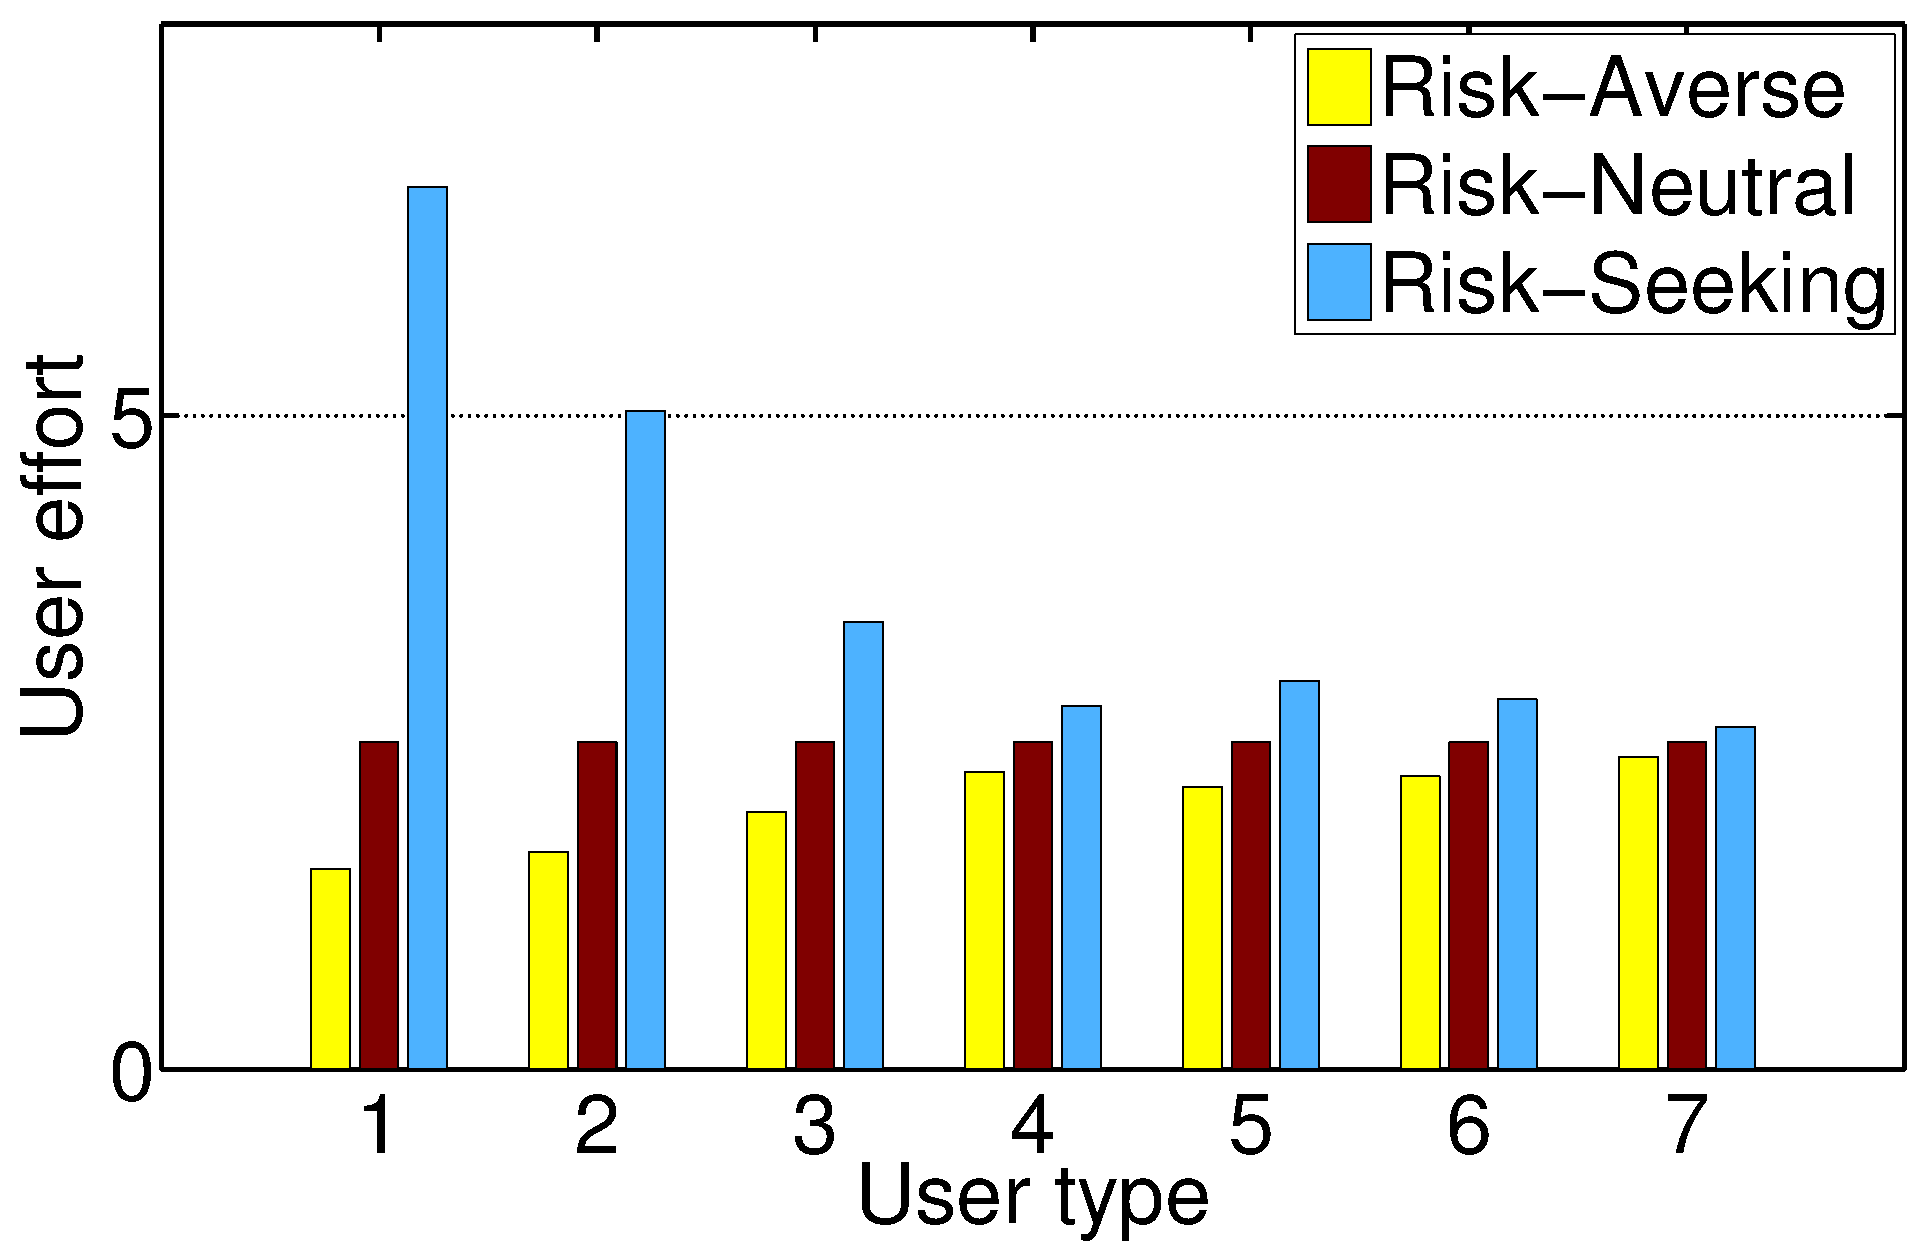
\includegraphics[width=\linewidth]{fig4}
	\caption{Example figure in Appendix~\ref{appendix:1}}
\end{figure}